\section{Ring Reducibility}
\label{sec:birkhoff}

Before 1913, the only known reductions of maps we're the reductions to triangulations and the reduction of multiply-connected regions to fewer regions (holed regions). In 1913, Birkhoff \cite{birkhoff} proved a new reduction result for \textit{rings} that seperate two parts of a map. This result spurred new developments in the reduction of graphs that opened the path towards reducible configurations and finally the proof of Appel and Haken in 1976.

\subsection{Rings and chains}

We will use the term \textit{map} to refer to a map of connected \textit{regions} that we wish to four-color. From such a map we can construct a \textit{planar graph} where each region represents a vertex. We will be working with planar graphs in all our proofs, but might sometimes mention maps for intuition.

Let $|G|$ be the number of vertices of $G$. Then we have the following well-known reduction to triangulations.

\begin{theorem}
\label{thm:triang}
    Given a planar graph $G$ with a non-triangular bounded face. Then the coloring of $G$ can be reduced to a graph on $H$ less vertices.
\end{theorem}
\begin{proof}
    A non-triangular bounded face of $G$ corresponds to a cycle of size greater than three in $G$. Combine any two non-neighboring vertices in this cycle to form a graph on one less vertex $H$. Given a coloring of $H$, we may color the two contracted vertices the same to obtain a coloring of $G$.
\end{proof}

Let us now define rings.

\begin{definition}
    A ring of $n$ vertices $R_n$ in a planar graph $G$ is an induced cycle of $G$ that encloses at least one vertex.
\end{definition}

The key property of rings is that they seperate the full graph $G$ in three parts $M_1$, $R$ and $M_2$. That is, $G$ is of the form $G = M_1 + R + M_2$ where the order of addition indicates how each part is connected to the other.

\begin{figure}[!ht]
    \centering
        \begin{tikzpicture}
        \draw[fill=white] (0,0) circle (2.5cm);
        \draw[fill opacity=0.4, pattern=crosshatch] (0,0) circle (1.5cm);
        \draw[fill=white] (0,0) circle (1cm);
        \node at (0, 1.25) {$R$};
        \node at (0, 2) {$M_2$};
        \node at (0, 0) {$M_1$};
    \end{tikzpicture}
    \caption{The graph $M_1 + R + M_2$.}
\end{figure}

To reduce a ring like this, we ideally want to color $M_1+R$ and $M_2+R$ in such a way that the colors on $R$ are the same. Then we can glue the two colorings together to form a coloring of $G$.

It might however, not always be possible to reduce a graph with a ring $R$ to $M_1+R$ and $M_2+R$. For a weaker result, we may try reducing to slightly larger graphs, $M_1+R+A_1$ and $M_2+R+A_2$ where $A_1$ and $A_2$ are two arbitrary graphs of at most $k$ vertices that are connected to $R_n$.

This is a weaker result, because if we allow $k$ to be big enough, we can simply set $A_1 = M_2$ and $A_2 = M_1$ to reduce to twice $M_1 + R + M_2$, which obviously has a common coloring on the ring. Let us define this generalization of ring reducibility.

\begin{definition}
    A ring $R_n$ is said to be k-reducible if for all planar graphs $G$ containing the ring $R_n$, the coloring of $G$ can be reduced to the coloring of $M_1+R_n+A_1$ and $M_1+R_n+A_2$ with $A_1$ and $A_2$ two arbitrary planar graphs on at most $k$ vertices that are connected to $R_n$.
\end{definition}

For example, the following is a trivial result.

\begin{example}
    The rings $R_1, R_2$ and $R_3$ are 0-reducible.
\end{example}

\begin{proof}
    The colorings only possible colorings on these rings (up to permutation) are $\{ a \}, \{ ab \}$ and $\{ abc \}$. Given a coloring of $M_1+R$ and $M_2+R$, we can simply permute the colors in both graphs to make the colorings agree on the ring. Hence we have 0-reducibility.
\end{proof}

Starting from the ring $R_4$, we briefly introduce two concepts to make the proof easier to follow. The first are Kempe-chains first introduced by Alfred Kempe.
\begin{definition}
    Given two colors $a,b$ and a coloring of a planar graph $G$. The $ab$-chain of a vertex $v$ in $G$ is the induced subgraph of $v$ and all vertices colored $a,b$ that are connected to $v$ directly or through other vertices colored $a,b$.
\end{definition}

In addition, we introduce a notation for writing down the colors on a ring $R$ and any chains that connect two vertices of the ring. We call these \emph{ring schemes}.

\begin{figure}[!ht]
    \centering
    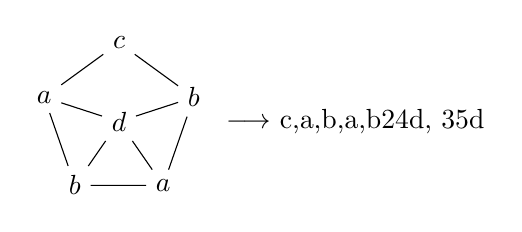
\begin{tikzpicture}
        \node (v1) at (0, 1) { $c$ };
        \node (v2) at (-0.95, 0.309) { $a$ };
        \node (v3) at (-0.56, -0.81) { $b$ };
        \node (v4) at (0.56, -0.81) { $a$ };
        \node (v5) at (0.95, 0.309) { $b$ };
        \node (x) at (0, 0) { $d$ };

        \draw (v1) -- (v2) -- (v3) -- (v4) -- (v5) -- (v1);
        \draw (v3) -- (x) -- (v5);
        \draw (v4) -- (x) -- (v2);

        \node (scheme) at (3, 0) { $\longrightarrow$ \scheme {c,a,b,a,b}{24d, 35d} };
    \end{tikzpicture}
    \\
    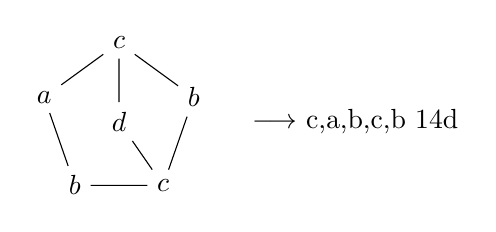
\begin{tikzpicture}
        \node (v1) at (0, 1) { $c$ };
        \node (v2) at (-0.95, 0.309) { $a$ };
        \node (v3) at (-0.56, -0.81) { $b$ };
        \node (v4) at (0.56, -0.81) { $c$ };
        \node (v5) at (0.95, 0.309) { $b$ };
        \node (x) at (0, 0) { $d$ };

        \draw (v1) -- (v2) -- (v3) -- (v4) -- (v5) -- (v1);
        \draw (v1) -- (x) -- (v4);

        \node (scheme) at (3, 0) { $\longrightarrow$ \scheme {c,a,b,c,b}{ 14d }};
    \end{tikzpicture}
    \\
    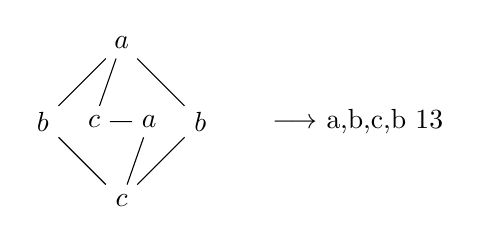
\begin{tikzpicture}
        \node (v1) at (0, 1) { $a$ };
        \node (v2) at (1, 0) { $b$ };
        \node (v3) at (0, -1) { $c$ };
        \node (v4) at (-1, 0) { $b$ };
        \node (x1) at (-0.35, 0) { $c$ };
        \node (x2) at (0.35, 0) { $a$ };

        \draw (v1) -- (x1) -- (x2) -- (v3);
        \draw (v1) -- (v2) -- (v3) -- (v4) -- (v1);
        \node (scheme) at (3, 0) { $\longrightarrow$ \scheme {a,b,c,b}{ 13 }};
    \end{tikzpicture}
    \caption{Examples of rings $R_4$ and $R_5$ with chains. A layout of chains on the ring can be indicated with the ring scheme notation. }
\end{figure}

The key property of ring schemes is that we may freely flip $ab$-chains for vertices that are seperated by a $cd$-chain, since these $ab$-chains can never be connected.

\begin{definition}
    A ring scheme $x$ implies another ring scheme $y$ if $y$ can be obtained from $x$ by flipping an $ab$-chain. In this case we write $x \compat y$.
\end{definition}

For example, in the earlier figure of a ring scheme on $R_4$ we have

\begin{equation*}
    \scheme{a,b,c,b}{{13}} \compat \scheme{a,b,c,d}{{13}}.
\end{equation*}

We will now use the concepts of chains and ring schemes to prove that the ring $R_4$ is 0-reducible and the ring $R_5$ 1-reducible.

\subsection{The ring $R_4$ is 0-reducible}

In this section we will prove the following theorem:

\begin{theorem}
    The ring $R_4$ is 0-reducible.
\end{theorem}
\begin{proof}

Let us consider the possible ring colorings I and II of the graphs $M_1+R_4$ and $M_2+R_4$. Since the ring in this case is a 4-cycle, we may color two of its vertices the same by Theorem \ref{thm:triang}. We can merge either $v_1$ and $v_3$ or $v_2$ and $v_4$ to obtain the colorings $a{*}a{*}$ and ${*}a{*}a$, where the ${*}$-vary per coloring.

If any of these two colorings in I and II are equal (up to permutation), we are done. Otherwise, we may assume that

\begin{equation}
    \{ abab \}\subset \I \quad \text{and}  \quad \{ abac, baca \} \subset \II.
\end{equation}

Now suppose that there is an $ad$-chain between $v_1$ and $v_3$ in $I(abab)$. We are allowed to flip the $bc$-chain of $v_4$ without affecting $v_2$ because the $ad$-chain in complementary colors seperates them. Thus we obtain

\begin{equation}
    \I(abab) = \scheme{a,b,a,b}{13d} \compat \II(abac)
\end{equation}

If there is no such $ad$-chain between $v_1$ and $v_3$, then likewise we are allowed to flip the $ad$-chain of $v_3$ without affecting $v_1$ to obtain

\begin{equation}
    \I(abab) = \scheme{a,b,a,b}{13d-} \compat \I(abcb) = \II(baca).
\end{equation}

In any case, we obtain a common coloring between I and II. Therefore the ring $R_4$ is 0-reducible.
\end{proof}

\subsection{The ring $R_5$ is 1-reducible}

A know result is that every planar graph has a vertex $v$ of degree at most 5. If we apply the reduction to triangulations, this means that the five vertices surrounding $v$ form the ring $R_5$. If $R_5$ we're 0-reducible, then every planar graph would be reducible and as a consequence, no minimal counterexamples could exist to the four color theorem.

This is an intuition as to why it might be hard to prove that $R_5$ is 0-reducible (we have tried). Instead we will prove the weaker 1-reducibility, this will turn out to be sufficient for subsequent work on the four color theorem.

\begin{theorem}
    The ring $R_5$ is 1-reducible.
\end{theorem}

\begin{proof}Let us consider the possible ring colorings I and II of $M_1 + R_5 + A_1$ and $M_2 + R_5 + A_2$. We must now take into account the graphs $A_1$ and $A_2$ on at most one vertex. The colorings depend on the amount of vertices in $A$

\emph{$A$ has one vertex}. In this case we have the sole vertex of $A$ connected to all vertices of the ring by definition. Because we assume four-colorability, the ring can only contain three colors and hence must be colored one of $\underline{c}abab$ where the vertex colored $\underline{c}$ is free to be any of the five vertices.

\emph{$A$ is empty}. In this case we have no vertices on the other side of the ring $R_5$. Because it is a 5-cycle, we may apply Theorem \ref{thm:triang} to merge any two opposing vertices thus coloring them the same. This results in five different colorings of the form $a{*}{*}a{*}$ where any two non-adjacent vertices may be colored $a$.

Therefore we assume the following colorings for I and II:

\begin{equation}
    \left\{ \begin{matrix}
        \text{one of}\;\underline{c}abab \; \text{with $c$ free}, \\
        \text{all of}\;a{*}{*}a{*} \; \text{with $a$  non-adjacent}
    \end{matrix}\right\} \subset \text{I, II}.
\end{equation}

Now we will prove that for these two sets, we can always deduce a common coloring on the ring $R_5$. To this end, we will prove two lemma's.

Let a vertex colored uniquely in one of $\underline{c}abab$ be called the \emph{marked vertex}, indicated by an underlined color. Let two colorings be called \emph{adjacent} if their marked vertices are adjacent.

\begin{lemma}
    \label{lem:r5_first}
    If I and II have a non-adjacent coloring, then they either have an adjacent coloring or a common coloring.
\end{lemma}

\begin{lemma}
    \label{lem:r5_second}
    If I and II have an adjacent coloring, then they have a common coloring.
\end{lemma}

\emph{Proof of Lemma \ref{lem:r5_first}}.
Let two non-adjacent colorings $\I(\underline{c}abab)$ and $\II(ab\underline{c}ab)$ be given. Suppose that a $bc$-chain connects $v_3$ and $v_5$ in $\II(ab\underline{c}ab)$. Then we obtain

\begin{equation}
    \label{eq:abcab}
    \II(ab\underline{c}ab) =\scheme{a,b,c,a,b}{35b} \compat \II(abcdb).
\end{equation}

If no such chain exists, then we may flip the $bc$-chain of $v_3$ to obtain

\begin{equation}
    \II(ab\underline{c}ab) = \scheme{a,b,c,a,b}{35b-} \compat \II(a\underline{c}bab) \;\; \text{adjacent to} \;\; \I(\underline{c}abab).
\end{equation}

Now to deal with the former coloring, we consider the coloring $\I({*}b{*}{*}b)$. The three unique possibilities for the colors lead to

\begin{equation}
    \begin{matrix*}[l]
        \I(abcdb) \quad\quad =&\II(abcdb) \; \text{from (\ref{eq:abcab}),}  \\
        \I(cbc\underline{d}b) \;\; \text{adjacent to}&\II(ab\underline{c}ab), \;  \\
        \I(db\underline{c}db) \quad\quad =&\II(ab\underline{c}ab).
    \end{matrix*}
\end{equation}

A similar argument holds for any other pair of non-adjacent colorings for I and II. Therefore we obtain either a common coloring or an adjacent coloring. These adjacent colorings are then treated by the second lemma $\qedsymbol$.

\vspace{1em}
\emph{Proof of Lemma \ref{lem:r5_second}}

Let two adjacent colorings $\I(\underline{c}abab)$ and $\II(a\underline{c}bab)$ be given. Suppose a $bd$-chain connects $v_3$ and $v_5$ in $\II(a\underline{c}bab)$. Then we obtain

\begin{equation}
    \II(a\underline{c}bab) = \scheme{a,c,b,a,b}{35d} \compat \I(\underline{c}abab).
\end{equation}

If no such chain exists, then we may flip the $bd$-chain of $v_3$ to obtain

\begin{equation}
    \label{eq:acdab}
    \II(a\underline{c}bab) = \scheme{a,c,b,a,b}{35d-} \compat \II(acdab).
\end{equation}

Now we consider the coloring $\I(a{*}{*}a{*})$. The three unique possibilities for the colors lead to

\begin{equation*}
    \begin{matrix*}[l]
        \I(acdab) \quad =& \II(acdab), \;\text{from (\ref{eq:acdab})},\\
        \I(ac\underline{d}ac) \; &\text{shifted two to right of $\I(\underline{c}abab)$}, \\
        \I(a\underline{c}dad) \quad =& \II(a\underline{c}bab).
    \end{matrix*}
\end{equation*}

By following this procedure, we end up with either a common coloring, or a coloring that is shifted two to the right.

We can repeat this procedure again with $\II(a\underline{c}bab)$ and $\I(ac\underline{d}ac)$, to obtain $\II(aba\underline{c}b)$. Another repetition yields another shifted coloring for I. Hence we obtain the pattern

\begin{equation}
    \I(\underline{c}abab) \rightarrow \I(ab\underline{c}ab) \rightarrow \I(abab\underline{c}) \rightarrow \I(a\underline{c}bab) = \II(a\underline{c}bab).
\end{equation}

A similar argument holds for any pair of adjacent colorings of I and II. Therefore, in all cases, we obtain a common coloring $\qedsymbol$.

\vspace{1em}
If the marked vertices are the same, we can simply permute colors to obtain a common coloring of I and II. Together with these two lemma's we will have covered all cases of marked vertices. Therefore the ring $R_5$ is 1-reducible.

\end{proof}

\subsection{Birkhoff graphs}

Now that we have proven two new reducibiliy results, we want to put them in the context of the four color theorem. In particular, we are interested in the nature of minimal counterexamples. Minimal counterexamples can not be reducible, because if they we're, we could reduce their coloring to a smaller graph that \emph{is} four colorable by minimality. Let $G$ be a minimal counterexample to the four-color theorem.

\emph{By 0-reducibility of $R_4$}, this means no vertex $v$ of $G$ can have four neighbours, since otherwise by triangulation, the neighbours of $v$ would form $R_4$ which is reducible.

\emph{By 1-reducibility of $R_5$}. In this case we can only reduce to a smaller graph if both sides of $R_5$, $M_1$ and $M_2$, have at least two vertices. Suppose the ring $R_5$ has a graph $M_1$ on one side, and a single vertex $v$ on the other. Then it is possible that one of our reduced graphs is $M_1 + R_5 + A_1$ with $|A_1|=1$, but this graph has exactly the same size as $G$. Therefore we did not achieve a size reduction. 

This means that we can only say with certainty that $G$ has no ring $R_5$ with more than two vertices on either side.
\\
A key definition in the three theorems for the four-color theorem is that of \emph{Birkhoff graphs}. These graphs are exactly the irreducible graphs $G$ we specified above.

\begin{definition}
    A Birkhoff graph $G$ is a planar triangulation without the ring $R_4$ and the ring $R_5$ of more than two vertices on either side.
\end{definition}

An equivalent definition is that of \emph{internally 6-connected triangulations}.

\begin{definition}
    An internally 6-connected triangulation is a graph $G$ where for any cutting set $X$ with $G\setminus X$ disconnected, $|X| \geq 6$ or $|X|=5$ with $G\setminus X$ having two components of which one is a single vertex.
\end{definition}

These two are equivalent because cuttings sets are the same as rings.
\\
Let us finish this section with one last result to test our intuition.

\begin{theorem}
    The four color theorem is equivalent to $R_5$ being 0-reducible.
\end{theorem}

\begin{proof}
\hfill\newline
$\Longrightarrow$ Suppose the four color theorem is true, then we know that any planar graph $M_1 + R_5 + M_2$ is four-colorable. Given such a four-coloring, we will obtain a common coloring for $M_1+R_5$ and $M_2+R_5$.\\
$\Longleftarrow$ Suppose that $R_5$ is 0-reducible. Given a minimal counterexample to the four color theorem $G$, then we have that there exists a vertex $v$ of degree at most five in $G$. Because $G$ is a triangulation, the neighbors of $v$ must form $R_5$. Because all rings smaller or equal to $R_5$ are 0-reducible, we may always reduce $G$ to two components $M_1+R_5$ and $v+R_5$, both of which are smaller than $G$. Therefore $G$ is four colorable and no minimal counterexample can exist.
\end{proof}

Since we already know that the four color theorem is true, we know that the ring $R_5$ is also 0-reducible. Because it might seem so easy to prove that $R_5$ is 0-reducible, it was in fact Alfred Kempe himself who gave the first false proof of the four color theorem. See \cite{kempe}.

Despite his failed proof, he continued on to introduce the concept of rings to mathematics on which this section is based, and these rings ended up at the heart of the four color theorem.